\documentclass[12pt, oneside]{article}

\usepackage[letterpaper, scale=0.8, centering]{geometry}
\usepackage{fancyhdr}
\setlength{\parindent}{0em}
\setlength{\parskip}{1em}

\pagestyle{fancy}
\fancyhf{}
\renewcommand{\headrulewidth}{0pt}
\rfoot{{\footnotesize Copyright Mia Minnes, 2024, Version \today~(\thepage)}}

\usepackage{titlesec}

\author{CSE105W24}

\newcommand{\instructions}{{\bf For all HW assignments:} Weekly homework 
may be done individually or in groups of up to 3 students. 
You may switch HW partners for different HW assignments. 
Please ensure your name(s) and PID(s) are clearly visible on the first page of your homework submission 
and then upload the PDF to Gradescope. If working in a group, submit only one submission per group: 
one partner uploads the submission through their Gradescope account and then adds the other group member(s) 
to the Gradescope submission by selecting their name(s) in the ``Add Group Members" dialog box. 
You will need to re-add your group member(s) every time you resubmit a new version of your assignment.
 Each homework question will be graded either for correctness (including clear and precise explanations and 
 justifications of all answers) or fair effort completeness. 
 For ``graded for correctness''
 questions: collaboration is allowed only with CSE 105 students in your group; 
 if your group has questions about a problem, you may ask in drop-in 
 help hours or post a private post (visible only to the Instructors) on Piazza.
 For ``graded for completeness''
 questions: collaboration is allowed with any CSE 105 students this quarter; 
 if your group has questions about a problem, you may ask in drop-in 
 help hours or post a public post on Piazza.

All submitted homework for this class must be typed. 
You can use a word processing editor if you like (Microsoft Word, Open Office, Notepad, Vim, Google Docs, etc.) 
but you might find it useful to take this opportunity to learn LaTeX. 
LaTeX is a markup language used widely in computer science and mathematics. 
The homework assignments are typed using LaTeX and you can use the source files 
as templates for typesetting your solutions.
To generate state diagrams of machines, we recommend using Flap.js
or JFLAP. Photographs of clearly hand-drawn diagrams may also be used. We recommend that you
submit early drafts to Gradescope so that in case of any technical difficulties, at least some of your
work is present. You may update your submission as many times as you'd like up to the deadline.


{\bf Integrity reminders}
\begin{itemize}
\item Problems should be solved together, not divided up between the partners. The homework is
designed to give you practice with the main concepts and techniques of the course, 
while getting to know and learn from your classmates.
\item You may not collaborate on homework questions graded for correctness with anyone other than your group members.
You may ask questions about the homework in office hours (of the instructor, TAs, and/or tutors) and 
on Piazza (as private notes viewable only to the Instructors).  
You \emph{cannot} use any online resources about the course content other than the class material 
from this quarter -- this is primarily to ensure that we all use consistent notation and
definitions (aligned with the textbook) and also to protect the learning experience you will have when
the `aha' moments of solving the problem authentically happen.
\item Do not share written solutions or partial solutions for homework with 
other students in the class who are not in your group. Doing so would dilute their learning 
experience and detract from their success in the class.
\end{itemize}

}

\newcommand{\gradeCorrect}{({\it Graded for correctness}) }
\newcommand{\gradeCorrectFirst}{\gradeCorrect\footnote{This means your solution 
will be evaluated not only on the correctness of your answers, but on your ability
to present your ideas clearly and logically. You should explain how you 
arrived at your conclusions, using
mathematically sound reasoning. Whether you use formal proof techniques or 
write a more informal argument
for why something is true, your answers should always be well-supported. 
Your goal should be to convince the
reader that your results and methods are sound.} }
\newcommand{\gradeComplete}{({\it Graded for completeness}) }
\newcommand{\gradeCompleteFirst}{\gradeComplete\footnote{This means you will 
get full credit so long as your submission demonstrates honest effort to 
answer the question. You will not be penalized for incorrect answers. 
To demonstrate your honest effort in answering the question, we 
expect you to include your attempt to answer *each* part of the question. 
If you get stuck with your attempt, you can still demonstrate 
your effort by explaining where you got stuck and what 
you did to try to get unstuck.} }

\usepackage{tikz}
\usetikzlibrary{automata,positioning,arrows}

\usepackage{amssymb,amsmath,pifont,amsfonts,comment,enumerate,enumitem}
\usepackage{currfile,xstring,hyperref,tabularx,graphicx,wasysym}
\usepackage[labelformat=empty]{caption}
\usepackage{xcolor}
\usepackage{multicol,multirow,array,listings,tabularx,lastpage,textcomp,booktabs}

\lstnewenvironment{algorithm}[1][] {   
    \lstset{ mathescape=true,
        frame=tB,
        numbers=left, 
        numberstyle=\tiny,
        basicstyle=\rmfamily\scriptsize, 
        keywordstyle=\color{black}\bfseries,
        keywords={,procedure, div, for, to, input, output, return, datatype, function, in, if, else, foreach, while, begin, end, }
        numbers=left,
        xleftmargin=.04\textwidth,
        #1
    }
}
{}

\newcommand\abs[1]{\lvert~#1~\rvert}
\newcommand{\st}{\mid}

\newcommand{\cmark}{\ding{51}}
\newcommand{\xmark}{\ding{55}}
 
\newcommand{\SUBSTRING}{\textsc{Substring}}
\newcommand{\REP}{\textsc{Rep}}
\newcommand{\blank}{\scalebox{1.5}{\textvisiblespace}}
 
\title{HW1CSE105W24: Homework assignment 1}
\date{Due: January 18th at 5pm (no penalty late submission until 8am next morning), via Gradescope}


\begin{document}
\maketitle
\thispagestyle{fancy}

{\bf In this assignment,}

You will practice reading and
applying the definitions of alphabets, strings, languages, Kleene star, and regular expressions.
You will use regular expressions and relate them to languages and finite automata.
You will use precise notation to formally define the state diagram of finite automata,
and you will use clear English to describe computations of finite automata informally.


{\bf Resources}: To review the topics 
for this assignment, see the class material from Week 1.
We will post frequently asked questions and our answers to them in a 
pinned Piazza post.

{\bf Reading and extra practice problems}: Sipser Section 0, 1.3, 1.1.
Chapter 1 exercises 1.1, 1.2, 1.3, 1.18, 1.23.

\instructions

You will submit this assignment via Gradescope
(\href{https://www.gradescope.com}{https://www.gradescope.com}) 
in the assignment called ``hw1CSE105W24''.

{\bf Assigned questions}
\begin{enumerate}[wide, labelwidth=!, labelindent=0pt]
\item\gradeCompleteFirst \textbf{Finding examples and edge cases} (12 points):

With $\Sigma_1 = \{0,1\}$ and 
$\Sigma_2 = \{a,b,c,d,e,f,g,h,i,j,k,l,m,n,o,p,q,r,s,t,u,v,w,x,y,z\}$
and $\Gamma = \{0,1,x,y,z\}$

    \begin{enumerate}
    \item Give an example of the shortest string over $\Sigma_1$ that is meaningful to you in some way, and explain 
    why it's meaningful to you.

    \item List all examples of strings of length $1$ over $\Sigma_2$ and explain why your list is exhaustive.

    \item Calculate the number of distinct strings of length 3 over $\Gamma$ and explain your calculation.

    \item With the ordering $x < y < z < 0 < 1$, list the first ten strings over $\Gamma$ in string order.

    \item Give an example of a finite set that is a language over $\Sigma_1$ and over $\Sigma_2$ and over $\Gamma$, 
    or explain why there is no such set.
    
    \item  Give an example of an infinite set that is a language over $\Sigma_1$  and over $\Gamma$, 
    or explain why there is no such set.

    \end{enumerate}

\item\gradeComplete \textbf{Regular expressions} (10 points):

    \begin{enumerate}
    \item Give three regular expressions that all describe the set of all strings over $\{a,b\}$ that have 
    even length. Ungraded bonus challenge: Make the expressions as different as possible!

    \item A friend tells you that each regular expression that has a Kleene star ($~^*$) describes an
    infinite language. Are they right? Either help them justify their claim or give a counterexample to disprove it
    and then fix the formula.

    \end{enumerate}

\item\gradeCorrectFirst \textbf{Functions over languages} (15 points):

For languages $L_1, L_2$ over the alphabet $\Sigma_1 = \{0,1\}$, we have the 
associated sets of strings
\[
    SUBSTRING(L_1) = \{ w \in \Sigma_1^* ~|~ \text{there exist } a,b \in \Sigma_1^* \text{ such that } awb \in L_1\}
\]
and 
\[
    L_1 \circ L_2 = \{ w \in \Sigma_1^* ~|~ w = uv \text{ for some strings } u \in L_1 \text{ and } v \in L_2 \}
\]
    \begin{enumerate}
    \item Specify an example language $A$ over $\Sigma_1$ such that 
    $A \neq \emptyset$ and yet $\SUBSTRING(A) = \emptyset$, 
    or explain why there is no such example. 
    A complete solution will include either (1) a precise and
    clear description of your example language $A$ 
    and a precise and clear description of
    the result of computing $\SUBSTRING(A)$ using relevant definitions 
    to justify this description and to justify the set equality with 
    $\emptyset$, or (2) a sufficiently general and correct argument
    why there is no such example, referring back to the relevant definitions.

    \item Specify example languages $B, C$ over $\Sigma_1$ such that 
    $B \neq \Sigma_1^*$ and $C \neq \Sigma_1^*$ and yet $B \circ C = \Sigma_1^*$, 
    or explain why there are no such examples. 
    A complete solution will include either (1) a precise and
    clear description of your example languages $B,C$ 
    and a precise and clear description of
    the result of computing $B \circ C$ using relevant definitions 
    to justify this description and to justify the set equality with 
    $\Sigma_1^*$, or (2) a sufficiently general and correct argument
    why there is no such example, referring back to the relevant definitions.

    \item Specify example {\bf finite} languages $L_1, L_2$ over $\Sigma_1$ such that 
    $L_1 \circ L_2 \neq L_1$ but $|L_1 \circ L_2| = |L_1|$, or 
    explain why there are no such examples.
    A complete solution will include either (1) a precise and
    clear description of your example languages $L_1, L_2$ 
    and a precise and clear description of
    the result of computing $L_1 \circ L_2$ using relevant definitions 
    to justify this description and to justify the cardinality claims and set (in)equality claims, 
    or (2) a sufficiently general and correct argument
    why there is no such example, referring back to the relevant definitions.
    \end{enumerate}


\item\gradeCorrect \textbf{Finite automata} (13 points):

Consider the finite automaton $(Q, \Sigma, \delta, q_0, F)$ whose state diagram is depicted below
\begin{center}
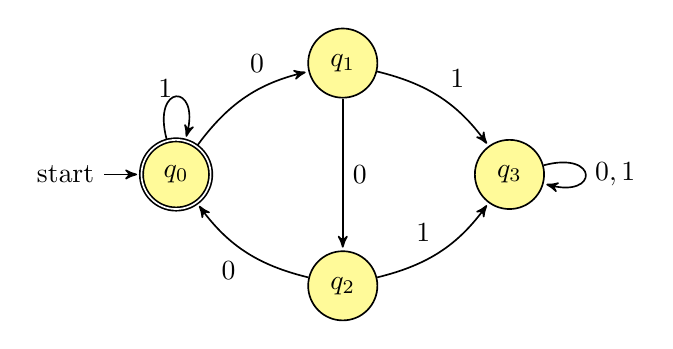
\begin{tikzpicture}[->,>=stealth',shorten >=1pt, auto, node distance=2cm, semithick]
\tikzstyle{every state}=[text=black, fill=yellow!40]

\node[initial,state, accepting] (q0)          {$q_0$};
\node[state]         (q1) [above right of=q0, xshift=20pt] {$q_1$};
\node[state]         (q2) [below right of=q0, xshift=20pt] {$q_2$};
\node[state]         (q3) [below right of=q1, xshift=20pt] {$q_3$};

\path (q0) edge  [loop above, near start] node {$1$} (q0)
        edge [bend left=20, near end] node {$0$} (q1)
    (q1) edge [bend left=0] node {$0$} (q2)
        edge [bend left=20] node {$1$} (q3)
    (q2) edge [bend left=20] node {$0$} (q0)
        edge [bend right=20] node {$1$} (q3)
    (q3) edge [loop right] node {$0,1$} (q3)
;
\end{tikzpicture}
\end{center}
where $Q = \{q_0, q_1, q_2, q_3\}$, $\Sigma = \{0,1\}$, and $F = \{q_0\}$, and $\delta: Q \times \Sigma \to Q$
is specified by the look-up table
\begin{center}
\begin{tabular}{c|cc}
        & $0$ & $1$ \\
    \hline
  $q_0$ & $q_1$ & $q_0$ \\
  $q_1$ & $q_2$ & $q_3$ \\
  $q_2$ & $q_0$ & $q_3$ \\
  $q_3$ & $q_3$ & $q_3$
\end{tabular}
\end{center}
    \begin{enumerate}
    \item  A friend tries to summarize the transition function with the formula
    \[
        \delta(q_i,x) = \begin{cases}
            q_0 &\text{ when $i=0$ and $x=1$} \\
            q_3 &\text{ when $0<i\leq 3$ and $x=1$}\\
            q_j &\text{ when $j = (i+1) \mod 3$ and $x=0$}
        \end{cases}
    \]
    Are they right? Either help them justify their claim or give a counterexample to disprove it and then 
    fix their formula.

    \item Give a regular expression $R$ so that $L(R)$ is the language 
    recognized by this finite automaton. Justify your answer by referring to the 
    definition of the semantics of regular expressions and computations of finite automata. 
    Include an explanation for why each string in $L(R)$ is accepted by the finite automaton {\it and}
    for why each string not in $L(R)$ is rejected by the finite automaton.

    \item  Keeping the same set of states $Q = \{q_0, q_1, q_2, q_3\}$, alphabet $\Sigma = \{0,1\}$, 
    same start state $q_0$, and same transition 
    function $\delta$, choose a new set of accepting states $F_{new}$ so that the new 
    finite automaton that results accepts at least one string that the original one rejected {\bf and} rejects
    at least one string that the original one accepted, or explain why there is no such choice of $F_{new}$.
    A complete solution will include either (1) a precise and
    clear description of your choice of $F_{new}$
    and a precise and clear the two example strings using relevant definitions 
    to justify them, or (2) a sufficiently general and correct argument
    why there is no such example, referring back to the relevant definitions.

    \end{enumerate}
    
    \end{enumerate}
\newpage

\title{HW2CSE105W24: Homework assignment 2}
\date{Due: February 1st at 5pm (no penalty late submission until 8am next morning), via Gradescope}



\maketitle
\thispagestyle{fancy}

{\bf In this assignment,}

You will practice designing multiple representations of regular languages and working with 
general constructions of automata to demonstrate the richness of the class of regular languages.
You will also distinguish between regular and nonregular languages using both closure arguments and the pumping lemma.


{\bf Resources}: To review the topics 
for this assignment, see the class material from Weeks 2-4.
We will post frequently asked questions and our answers to them in a 
pinned Piazza post.

{\bf Reading and extra practice problems}:  
Sipser Chapter 1, Section 2.2. 
Chapter 1 exercises 1.4, 1.5, 1.6, 1.7, 1.8, 1.9, 1.10, 1.11, 1.12, 1.14, 1.15, 
1.16, 1.17, 1.19, 1.20, 1.21, 1.22, 1.29, 1.30. Chapter 1 problems 1.49, 1.50, 1.51.

\instructions

You will submit this assignment via Gradescope
(\href{https://www.gradescope.com}{https://www.gradescope.com}) 
in the assignment called ``hw2CSE105W24''.

{\bf Assigned questions}
\begin{enumerate}[wide, labelwidth=!, labelindent=0pt]
\item \textbf{Number representations} (12 points):
Integers can be represented using base $b$ expansions, for a convenient choice of base $b$: 
for $b$ an integer greater than $1$ and $n$ a positive integer, 
the {\bf base $b$ expansion of $n$}  is defined to be
\[
(a_{k-1} \cdots a_1 a_0)_b
\]
where $k$ is a positive integer, $a_0, a_1, \ldots, a_{k-1}$ 
are nonnegative integers less than $b$, $a_{k-1} \neq  0$, and
\[
n =  \sum_{i=0}^{k-1} a_{i} b^{i}
\]

Notice: {\it The base $b$ expansion of a positive integer $n$ is a string over the alphabet 
$\{x \in \mathbb{Z} \st 0 \leq x < b\}$
whose leftmost character is nonzero.}

An important property of base $b$ expansions of integers is that, for each integer $b$ greater than $1$,
each positive integer $n = (a_{k-1} \cdots a_1 a_0)_b$, and each nonnegative integer $a$ less than $b$, 
\[
    bn + a = (a_{k-1} \cdots a_1 a_0a)_b
\]
In other words, shifting the base $b$ expansion to the left results in multiplying the integer value by the base.
In this question we'll explore building deterministic finite automata that recognize 
languages that correspond to useful sets of integers.

    \begin{enumerate}
    \item\gradeCorrectFirst Design a DFA that recognizes the set of binary (base $2$) expansions of 
    positive integers that are powers of $2$. A complete solution will include the state diagram of your DFA and 
    a brief justification 
    of your construction by explaining the role each state plays in the machine, as well as a brief 
    justification about how the strings accepted and rejected by the machine connect to the specified language.

    {\it Hints}: (1) A power of $2$ is an integer $x$ that can be written as $2^y$ for some nonnegative integer $y$, 
    (2) the DFA should accept the strings $100$, $10$ and $100000$ and should reject the 
    strings $010$, $1101$, and $\varepsilon$ (can you see why?).

    \item\gradeCompleteFirst Consider arbitrary positive integer $m$. Design a DFA that recognizes the 
    set of binary (base $2$) expansions of positive integers that are multiples of $m$. A complete solution will
    include the formal definition of your DFA (paramterized by $m$) and a brief justification of your 
    construction by explaining the role each state plays in the machine, as well as a brief 
    justification about how the strings accepted and rejected by the machine connect to the specified language.

    {\it Hints}: (1) Consider having a state for each possible remainder upon division by $m$.
     (2) To determine transitions, notice that reading a new character will shift what we already read over by
     one slot.

    \item\gradeCorrect Choose a positive integer $m_{0}$ between $4$ and $8$ (inclusive) and draw the state diagram
    of a DFA recognizing the language over $\{0,1,2\}$ $$\{ w \in \{0,1,2\}^* \mid w \text{ is a base $3$ expansion of a positive 
    integer that is a multiple of $m_0$}\}$$
    A complete solution will include the state diagram of your DFA and 
    a brief justification 
    of your construction by explaining the role each state plays in the machine, as well as a brief 
    justification about how the strings accepted and rejected by the machine connect to the specified language.
    \end{enumerate}

    {\it Bonus extension to think about (ungraded):} Which other languages related to sets of integers 
    can be proved to be regular using a similar strategy? 


\item\textbf{Multiple representations} (10 points):
For any language $L \subseteq \Sigma^*$, recall that we define its \emph{complement} as 
$$\overline{L} := \Sigma^* - L = \{w \in \Sigma^* \mid w \notin L\}$$ That is, the complement of $L$ 
contains all and only those strings which are not in $L$. Our notation for regular expressions does not 
include the complement symbol. However, 
it turns out that the complement of a language described by a regular expression is guaranteed to also be describable by a 
(different) regular expression. For example, over the alphabet $\Sigma = \{0,1\}$, the complement of the language described 
by the regular expression $\Sigma^* 0$ is described by the regular expression $\varepsilon \cup \Sigma^*1$
because any string that does not end in $0$
must either be the empty string or end in $1$.

For each of the regular expressions $R$ over the alphabet $\Sigma = \{a,b\}$ below, write the regular 
expression for~$\overline{L(R)}$. Your regular expressions may use the symbols
$\varnothing$, $\varepsilon$, $a$, $b$, and the 
following operations to combine them: union, concatenation, 
and Kleene star.

Briefly justify why your solution for each part works by giving plain English descriptions of the language 
described by the regular expression and of its complement and connecting them to the regular 
expression via relevant definitions. An English description that is more 
detailed than simply negating the description in the original language will likely be helpful in the justification.

Alternatively, you can justify your solution by first designing a DFA that recognizes $L(R)$, 
using the construction from class and the book to modify this DFA to get a new DFA that recognizes~$\overline{L(R)}$, 
and then applying the constructions from class and the book to convert this new DFA to a regular expression.

For each part of the question, clearly state which approach you're taking and include enough intermediate
steps to illustrate your work.


\begin{enumerate}
    \item\gradeCorrect $a^*b^*$
    \item\gradeCorrect $(a \cup b) a b^*$
\end{enumerate}


\item\textbf{Applying general constructions} (12 points):
In this question, you'll practice working with formal general constructions
for NFAs and translating between state diagrams and formal definitions.
Consider the following general construction: Let $N_1 = (Q, \Sigma, \delta_1, q_1, F_1)$ be a NFA
and assume that $q_0 \notin Q$.
Define the new NFA $N_2 = (Q \cup \{q_0\}, \Sigma, \delta_2, q_0, \{q_1\})$ where 
$$\delta_2: (Q \cup \{q_0\}) \times \Sigma_\varepsilon \to \mathcal{P} (Q \cup \{q_0\})$$ is defined by
\[
    \delta_2 (q,a) = \begin{cases}
        \{ q' \in Q \mid q \in \delta_1(q',a)\} &\text{if $q \in Q$, $a \in \Sigma_{\varepsilon}$} \\
        F_1 &\text{if $q =q_0$, $a = \varepsilon$}\\
        \emptyset &\text{if $q = q_0$, $a \in \Sigma$}
    \end{cases}
\]

\begin{enumerate}
\item\gradeCorrect Illustrate this construction by defining a specific example NFA $N$ and applying the 
construction above to create a new NFA. Your example NFA should
\begin{itemize}
    \item Have exactly three states (all reachable from the start state),
    \item Have at least one spontaneous move (arrow labelled $\varepsilon$),
    \item Accept at least one string and reject at least one string, and
    \item Not have any states labelled $q_0$.
\end{itemize}
Apply the construction above to create the new NFA. A complete submission 
will include the state diagram of your example NFA $N$ and the state diagram of the NFA resulting 
from this construction.
\item\gradeCorrect Use Theorem 1.39 on page 55 of the book (see also page 7 in Week 3 notes) to construct a 
DFA equivalent to your example NFA $N$ from part (a).
A complete submission 
will include the state diagram of your example NFA $N$ and the state diagram of the DFA resulting 
from this construction, with the correct state labels for this DFA. You may prune the DFA so that only the ``macro-states''
reachable from the start state are included.
\item \gradeComplete Explain the relationship between $N_1$ and $N_2$ in the general construction.
Give an example string that is accepted by your example NFA $N$ and is rejected by the NFA that results from 
applying the general construction that illustrates this relationship, or explain why there is no such example string.

\end{enumerate}


\item \textbf{Pumping} (8 points):

\begin{enumerate}
\item\gradeCorrect Give an example of a language
over the alphabet $\{0,1\}$ that has cardinality $3$ and for which $5$ is a pumping length
and $4$ is not a pumping length.  A complete solution will give a clear and precise
description of the language, a justification for why $5$ is a pumping length, and a 
justification for why $4$ is not a pumping length. Is this language regular?
\item\gradeComplete Consider the following attempted ``proof" that the set 
$$X = \{ uw \mid \text{$u$ and
$w$ are strings over $\{0,1\}$ and have the same length} \}$$
is nonregular.
\begin{quote}
``Proof" that $X$ is not regular using the Pumping Lemma: Let $p$ be 
an arbitrary positive integer. We will show that $p$ is not a pumping length for $X$. 

Choose $s$ to be the string $1^p 0^p$, which is in $X$ because
we can choose $u = 1^p$ and $w = 0^p$ which each have length $p$.
Since $s$ is in $X$ and has length greater than or equal to $p$, if $p$ were to be a
pumping length for $X$, $s$ ought to be pump'able. 
That is, there should be a way of dividing $s$ into parts $x,y,z$ where $s=xyz$,
$|y| >0$, $|xy| \leq p$, and for each $i \geq 0$, $xy^iz \in X$.
Suppose $x,y,z$ are such that $s = xyz$, $|y| > 0$ and $|xy| \leq p$.
Since the first $p$ letters of $s$ are all $1$ and $|xy| \leq p$, we know
that $x$ and $y$ are made up of all $1$s.  If we let $i=2$, we get 
a string $xy^iz$ that is not in $X$ because repeating $y$ twice adds $1$s to 
$u$ but not to $w$, and strings in $X$ are required to have $u$ and $w$ be the same
length. Thus, $s$ is not pumpable (even though it should have been if $p$ were to be a pumping length)
and so $p$ is not a pumping length for $X$.  Since $p$ was arbitrary, we have
demonstrated that $X$ has no pumping length.  By the Pumping Lemma, this implies that 
$X$ is nonregular.
\end{quote}
Find the (first and/or most significant) logical error in the ``proof" and describe why it's wrong.
Then, either prove that the set is actually regular (by finding a regular expression that describes it or 
a DFA/NFA that recognizes it, and justifying why) {\bf or} fix the proof so that it is logically sound.

\item\gradeComplete In class and in the reading so far, we've seen the following examples of nonregular sets:
\begin{multicols}{3}
\begin{center}
$\{ 0^n 1^n ~|~ n \geq 0 \}$
$$\{ 0^n 1^n ~|~ n \geq 2 \}$$
$$\{ 0^n 1^m ~|~  0 \leq n \leq m \}$$
$$\{ 0^n 1^m ~|~ 0 \leq m \leq n \}$$
$$\{ 0^i 1^{2i} ~|~ 0 \leq i \}$$
$$\{ 0^i 1^{i+1} ~|~ 0 \leq i \}$$
$$\{ 0^n 1^m 0^n ~|~n,m \geq 0\}$$
$$\{ w \in \{0,1\}^* ~|~w = w^R\}$$
$$\{ w w^R ~|~ w \in \{0,1\}^*\}$$
\end{center}
\end{multicols}
Modify one of these sets in some way and use the Pumping Lemma to prove that the resulting set is still nonregular.

\end{enumerate}

\item\textbf{Regular and nonregular languages} (8 points):
In Week 2's review quiz, we saw the definition that a set $X$ is said to be 
{\bf closed under an operation} if, for any elements in
$X$, applying to them gives an element in $X$. For example, the set of
integers is closed under multiplication because if we take any two
integers, their product is also an integer .

Prove or disprove each closure claim statement below about the class of regular languages
and the class of nonregular languages.
Your arguments may refer to theorems proved in the textbook and class, and if they do, should 
include specific page numbers and references (i.e.\ write out the claim that was proved in the book 
and/or class).

Recall the definitions we have: 

For languages $L_1, L_2$ over the alphabet $\Sigma_1 = \{0,1\}$, we have the 
associated sets of strings
\[
   SUBSTRING(L_1) = \{ w \in \Sigma_1^* ~|~ \text{there exist } a,b \in \Sigma_1^* \text{ such that } awb \in L_1\}
\]
and 
\[
   L_1 \circ L_2 = \{ w \in \Sigma_1^* ~|~ w = uv \text{ for some strings } u \in L_1 \text{ and } v \in L_2 \}
\]
\begin{enumerate}

    \item \gradeComplete The set of regular languages over $\{0,1\}$ is closed under set-wise concatenation.

    \item \gradeComplete The set of nonregular languages over $\{0,1\}$ is closed under set-wise concatenation.
 
   \item \gradeComplete The set of regular languages over $\{0,1\}$ is closed under the $SUBSTRING$ operation.

   \item \gradeComplete The set of nonregular languages over $\{0,1\}$ is closed under the $SUBSTRING$ operation.
\end{enumerate}
\end{enumerate}
\newpage
\titleformat{\subsubsection}[runin]
   {\normalfont\bfseries}{}{}{}
   
\title{ProjectCSE105W24: Project}
\date{Due February 22 at 5pm (no penalty late submission until 8am next day)}


\maketitle

\thispagestyle{fancy}


The CSE 105 project is designed for you to go deeper and extend your work on assignments 
and to explore an application of your choosing. 
The project is an individual assignment and has two tasks: 

Task 1: Implementing the construction that converts NFA to DFA, and

Task 2: Illustrating the theorem that every regular language is decidable


\subsubsection*{What resources can you use?} This project must be completed individually, 
without any help from other people, including the course staff (other than logistics support if 
you get stuck with screencast).
You can use any of this quarter's CSE 105 offering (notes, readings, class videos, homework feedback). 
Tools for drawing state diagrams (like Flap.js and JFLAP) can be used to help draw the diagrams 
in the project too.
These resources should be more than enough.
If you are struggling to get started and want to look elsewhere online, 
you must acknowledge this by listing and citing any resources you consult 
(even if you do not explicitly quote them), including any large-language model style resources. 
Link directly to them and include the name of the author / video creator, 
any search strings or prompts you used, and the reason you consulted this reference.

The work you submit for the project needs to be your own. Again, you shouldn't need to look anywhere 
other than this quarter's material and doing so may result in definitions or notations that 
conflict with our norms in this class so think carefully before you go down this path.

If you get stuck on any part of the project, we encourage you to focus on communicating what you think 
the question might mean, including bringing an example from class or homework you think might be relevant, and 
include any submission any aspect where you're unsure. Clear communication about these
theoretical ideas and their applications ia one of the main goals of the project.

{\bf Submitting the project} You will submit a PDF plus a video file for the first task and a PDF for the 
second task. All file submissions will be in Gradescope.

\newpage
\subsubsection*{Task 1: Implementing a construction}

Nondeterminism is a useful theoretical concept because it can make designs simpler and more modular. 
However, our actual devices are deterministic. In this part of the project, you'll choose a 
language that can be represented using nondeterminism in some interesting way, then illustrate
the construction that converts NFA to DFA for this example.

Specifically:

\begin{enumerate}
\item Choose an alphabet $\Sigma$ for this entire first task of the project.
\item Write a program in Java, Python, JavaScript, C++ , or another programming language of your choosing
 that takes as input a representation of an NFA over this alphabet and outputs
 a representation of a DFA over this alphabet that recognizes the same language. 
 You get to choose the way NFA and DFA are represented, so long as it is
 general enough to represent any NFA and any DFA over this alphabet. For simplicity: you can 
 restrict your attention to NFA **without spontaneous moves** (in other words, where the transition function 
 has domain $Q \times \Sigma$ when $Q$ is the set of states of the NFA). Informally, this means
 that the nondeterminism is coming from there being zero, one, or more arrows coming out of each state
 for each character in the alphabet and there are no arrows with $\varepsilon$ labels.

 If you would like, you may use aids such as co-pilot or ChatGPT to help you write this program. 
 However, you should test the code that is produced and be able to explain what it is doing. 
 As a header in your code file, include a comment block describing any resources that were used to 
 help generate your code.

 Whenever your program is run, it should display a representation of the input NFA and 
 of the output DFA of the run.

\item To demonstrate your program, design a NFA over $\Sigma$ with three states and with no spontaneous moves 
where the language of the NFA is neither $\emptyset$ nor $\Sigma^*$ and draw its state diagram.
Your NFA should use nondeterminism in some way. In other words, the state diagram you draw can't 
already be the state diagram of a DFA. Run your program with the NFA you just designed to output a 
representation of an equivalent DFA and
demonstrate its design and the test case on video.

\end{enumerate}

{\bf Checklist for submission}

For this task, you will submit a PDF plus a video file.

The PDF should include: 
\begin{itemize}
   \item Clear specification of alphabet and state diagram of chosen three-state NFA.
   \item Documentation for program converting NFA to DFA: include a description of how NFA and DFA are 
   represented in the program and give instructions for running it.
   \item Printout of code for program converting NFA to DFA.
   \item Screen shots of demonstration of running your program on your chosen NFA, including the representation
   of the output DFA.
   \item Solution is typed or clearly hand drawn with precise language and notation for all terms.
\end{itemize}

Presenting your reasoning and demonstrating it via screenshare are important skills that also 
show us a lot of your learning. Getting practice with this style of presentation is a good thing 
for you to learn in general and a rich way for us to assess your skills. 
To demonstrate your work, you will create a 3-5 minute screencast video with the following components:

\begin{itemize}
\item Start with your face and your student ID for a few seconds at the beginning, 
and introduce yourself audibly while on screen. You don't have to be on camera for the 
rest of the video, though it's fine if you are. We are looking for a brief confirmation that 
it's you creating the video and doing the work you submitted.
\item Present the NFA you will be working with. Your video should include a clear and precise 
explanation of why the language of this NFA is not empty and also not the set of all strings over $\Sigma$.
\item Show on the screen and explain the code for your program, including the software design choices you made
(e.g. which data structures are you using, etc.) and any resources you used. The video 
should clearly describe which programming language was chosen 
for the implementation and gives the reasons why.
\item Show on the screen and explain the representation of the NFA that you will input to the program.
\item Demonstrate running your code on your example input. The video should include screencasts of 
running the code live.
Explain why the output of your program is what you would expect, by connecting the output of the 
program to a DFA and discussing which strings are accepted / rejected by this DFA.
\item Logistics: video needs to load correctly, be between 3 and 5 minutes, 
show your face and ID, and you introduce yourself 
audibly while on screen.
\end{itemize}

{\bf Note}: Clarity and brevity are both important aspects of your video.  In previous years, we've seen 
students speed up their videos to get below the 5 minute upper bound. This is ok so long as it doesn't 
compromise clarity.

\subsubsection*{Task 2: Illustrating a theorem}

In this part of the project, you'll choose a pattern in an application you care about, 
define it precisely, build a DFA that recognizes it, and then build the related Turing machine
that proves that the language encoding this pattern is decidable.

First, pick {\bf one} application for your example. 
Here are some ideas to get you started - but you can choose to go in a different direction.
\begin{itemize}
\item Data validation for input in text files (e.g. emails with specific domains, dates in specific formats, PIDs in a class list, etc.)
\item Finding ASCII codes for punctuation in a binary file.
\item The CDC recommended procedure for hand washing (Refer to the guidelines from the CDC here 
\href{https://www.cdc.gov/handwashing/index.html}{https://www.cdc.gov/handwashing/index.html} in your explanation. 
You might find the first example in chapter 1 about automatic door controllers helpful when starting your design.)
\item See more ideas here:
\href{https://theory-cs.github.io/files/practical-applications-of-theory-of-computation.pdf}{https://theory-cs.github.io/files/practical-applications-of-theory-of-computation.pdf}
\end{itemize}
Then:
\begin{enumerate}
   \item In a paragraph or so, give the context for your chosen application and why you chose it.
   \item Specify the alphabet for your example and write a precise (mathematical and/or English) description of a set of strings over 
   this alphabet that is relevant to this application, and include a sentence or so justifying why this set is 
   important and relevant.
   \item Give one example of a string over this alphabet in this set and a string 
   over this (same) alphabet not in this set, and explain why you 
   chose these example strings.
   \item Design a DFA that recognizes this language. Clearly draw and label the state diagram 
   of this DFA and briefly justify why your design works by describing the role of each state of the DFA and 
   relating it to a plain English description of the language you picked.
   \item Use the construction in the proof that all regular languages are decidable
   (informally described in Theorem 4.1 in the book) to build a Turing machine
   that simulates your DFA. Hint: your Turing machine will have exactly two more states than your DFA.
   Draw the state diagram of your Turing machine.
   \item For one of the strings from step 4., draw a representation of the computation of your 
   Turing machine on this string.
   Remember that to describe the computation of a Turing machine, we need to include the contents of the 
   tape, the state of the machine, and the location of the read/write head at each step in the computation.
   In class we've drawn pictures to represent the configuration of the machine at each step 
   in a computation.  You may do so or you may choose to describe these configurations in words.
\end{enumerate}
{\bf Checklist for submission}
\begin{itemize}
   \item Solution typed or clearly hand-written/drawn with precise language and notation for all terms and complete, correct, and clear justification.
   \item Each of the six steps is complete and included in the PDF, with precise language and notation for all
    terms and complete, correct, and clear justification.

\end{itemize}


\subsubsection*{Your video:} You may produce screencasts 
with any software you choose. 
One option is to record yourself with Zoom; a tutorial on how to use 
Zoom to record a 
screencast (courtesy of Prof. Joe Politz)  is here: 

\url{https://drive.google.com/open?id=1KROMAQuTCk40zwrEFotlYSJJQdcG_GUU}.

The video that was produced from that recording session in Zoom is here:

\url{https://drive.google.com/open?id=1MxJN6CQcXqIbOekDYMxjh7mTt1TyRVMl}

Please send an email to the instructors 
(minnes@ucsd.edu) if you have 
concerns about  the video / screencast components of this project or 
cannot complete projects in this style for some reason.

\newpage

\end{document}